\documentclass[conference]{IEEEtran}
\IEEEoverridecommandlockouts
% The preceding line is only needed to identify funding in the first footnote. If that is unneeded, please comment it out.
\usepackage{cite}
\usepackage{amsmath,amssymb,amsfonts}
\usepackage{algorithm}
\usepackage{algorithmic}
\usepackage{graphicx}
\usepackage{textcomp}
\usepackage{xcolor}
\usepackage{enumerate}
\def\BibTeX{{\rm B\kern-.05em{\sc i\kern-.025em b}\kern-.08em
    T\kern-.1667em\lower.7ex\hbox{E}\kern-.125emX}}
\begin{document}

\title{Adaptive Metamorphic Testing*\\
%{\footnotesize \textsuperscript{*}Note: Sub-titles are not captured in Xplore and
%should not be used}
%\thanks{Identify applicable funding agency here. If none, delete this.}
\thanks{The National Natural Science Foundation of China (under Grant No. 61872039),
the Beijing Natural Science Foundation (Grant No. 4162040),
the Aeronautical Science Foundation of China (Grant No. 2016ZD74004), and
the Fundamental Research Funds for the Central Universities (Grant No. FRF-GF-17-B29).}
}

\author{\IEEEauthorblockN{1\textsuperscript{st} Chang-ai~Sun,~\IEEEmembership{Senior Member,~IEEE,}}
\IEEEauthorblockA{\textit{School of Computer and Communication Engineering} \\
\textit{University of Science and Technology Beijing}\\
Beijing, China \\
casun@ustb.edu.cn}
\and
\IEEEauthorblockN{2\textsuperscript{nd} Hepeng~Dai}
\IEEEauthorblockA{\textit{School of Computer and Communication Engineering} \\
\textit{University of Science and Technology Beijing}\\
Beijing, China \\
daihepeng@sina.cn}
\and
\IEEEauthorblockN{3\textsuperscript{rd} Tsong Yueh~Chen}
\IEEEauthorblockA{\textit{Faculty of Information and Communication Technologies} \\
\textit{Swinburne University of Technology Australia}\\
Melbourne, Australia \\
tychen@swin.edu.au}
\and
\IEEEauthorblockN{4\textsuperscript{th} Given Name Surname}
\IEEEauthorblockA{\textit{dept. name of organization (of Aff.)} \\
\textit{name of organization (of Aff.)}\\
City, Country \\
email address}
}

\maketitle

\begin{abstract}
  Metamorphic testing (MT) is a promising technique to alleviate the oracle problem, which fist defines metamorphic relations (MRs) used to generate new test cases (i.e. follow-up
  test cases) from the original test cases (i.e. source test cases). Both source and follow-up test cases are executed and their results are verified against the relevant MRs.
  Up to now, in terms of improving the efficiency of MT, researchers have focused their efforts on generating or selecting better MRs, while ignoring the impact of source test
  cases.
  Most of MT techniques employ random testing strategy (RT) to select source test cases. Although RT is simple and easy to use, it may not be efficient because RT does not use
  any information of the software under test. This study aims to improve the efficiency of MT through controlling the execution process of MT, and proposes a adaptive metamorphic
  testing (AMT) technique based on partition. We conduct a empirical study where AMT is employed to test three real-life programs. The results of empirical study show the
  feasibility of AMT, and AMT outperforms RT on enhancing the efficiency of MT.
\end{abstract}

\begin{IEEEkeywords}
metamorphic testing, control test process, partition
\end{IEEEkeywords}

\section{Introduction}
\label{section:introduction}
Test result verification is an important part of software testing. A test oracle \cite{weyuker1982testing} is mechanism that can exactly decide whether or not the output
produced by a programs is correct. However, there are situations, where it is difficult to decide whether the result of the software under test (SUT) agrees with the expected
result. This situation is known as oracle problem \cite{barr2015oracle, patel2018mapping}.

Metamorphic testing (MT) \cite{chen1998metamorphic, chen2018metamorphic} is one of several techniques to alleviate oracle problem. MT first define metamorphic relations (MRs)
through using some properties of SUT. Then, MRs are used to generate new test cases called follow-up test cases from original test cases known as source test cases. Next,
both follow-up and source test cases are executed and their result are verified against the corresponding MRs.

Obviously, the efficiency of MT in detecting faults relay on the quality of MRs and the source test cases. There have been vast studies to investigate generate and select
good MRs \cite{chen2004case, cao2013correlation, chen2004metamorphic, sun2011metamorphic, chen2014metric, xie2016looking}. However, Researchers ignore the impact of source
test cases on the efficiency of MT. Random testing (RT) that randomly selects test cases from input domain (which refers to the set of all possible inputs of SUT), is most
commonly used technique in MT \cite{segura2016survey}. Although RT is simple to implement, RT does not make use of any information about SUT, or the test history. Thus,
RT may be inefficient in some situations.

In contrast to RT, partition testing (PT) attempts to generate test cases in a more ��systematic�� way, aiming to use fewer test cases to reveal more faults. When conducting
PT, the input domain of the SUT is divided into disjoint partitions, with test cases then selected from each and every one. Each partition is expected to have a certain degree
of homogeneity��test cases in the same partition should have similar software execution behavior. Ideally, a partition should also be homogeneous in fault detection: If one
input can reveal a fault, then all other inputs in the same partition should also be able to reveal a fault.

%Based on different intuitions, RT and PT have their own advantages and disadvantages. It is likely that they can be complementary to each other, detecting different faults.
%Therefore, it is intuitively appealing to investigate the their integration. Based on software cybernetics \cite{cai2002optimal}, Cai et al. proposed dynamic random testing (DRT)
%\cite{cai2009random} that takes advantages of testing information to control the testing process, improving both RT and PT. DRT attempts to dynamically adjust testing profile:
%If a test case from a partition $s_i$ reveals a fault, the corresponding $p_i$ will be increased by a constant $\epsilon$; otherwise, it is decreased by $\epsilon$.


This paper proposes a adaptive metamorphic testing framework based on PT to improve the efficiency of MT. We investigate how to make use of feedback information to control
the execution process of MT, and conduct an empirical study. The paper makes the following contributions:

\begin{itemize}
  \item
  \emph{An adaptive metamorphic testing framework} which shows how to control the execution process of MT. The framework combines the basic principle of MT with the software
  cybernetics \cite{cai2002optimal}.
  \item
  \emph{An MRs-centric adaptive metamorphic testing technique (M-AMT)} which adds a feedback mechanism to control the execution process of MT. First, M-AMT randomly selects an
  MR to generate source and follow-up test cases of related input partitions, and then updates the test profile of input partitions according to the results of test execution.
  Second, a partition is selected according to updated test profile, and an MR is randomly selected from the set of MRs whose source test cases belong to selected partition.
  \item
  \emph{A supporting tool of adaptive metamorphic testing called APT2MT} has been developed to further improve the automation of the proposed AMT, which has features such as
  termination condition setting, partition setting, test execution, and test report generation.
  \item
  \emph{An empirical study} that has been conducted to evaluate the fault detection efficiency of the proposed AMT , where three Java programs are selected as subjects to
  compare the performance of traditional MT and AMT in terms of fault detection efficiency and time overhead in test case selection.
\end{itemize}

The rest of the paper is organized as follows. Section \ref{section:background} introduces underlying concepts related to MT, adaptive partition testing, and mutation analysis.
Section \ref{section:motivation} gives the motivation of this study. Section \ref{section:amt} presents a framework of MT for Web services. Section \ref{section:empirical}
reports a case study where MT is employed to test a Web service implementing the electronic payment. Related work is discussed in Section \ref{section:related}.

\section{Background}
\label{section:background}
\subsection{Metamorphic Testing}
\label{section:mt}
A test oracle is a mechanism used to verify the correctness of outputs of a program \cite{weyuker1982testing}. However, there are test oracle problem
\cite{barr2015oracle, patel2018mapping} in testing, that is, there are not an oracle or the application of such an oracle is very expensive. In order to alleviate the test oracle,
several techniques have been proposed such as N-version testing \cite{brilliant1990performance}, metamorphic testing (MT) \cite{chen1998metamorphic},
assertions \cite{sim2014eliminating}, machine learning \cite{chan2009pat}, etc. Among of them, MT obtains metamorphic relations (MRs) according to the properties of software
under test (SUT). MRs are used to generate follow-up test cases from source test cases, then the both source and follow-up test cases are executed, and their results are
verified against the corresponding MRs. If an MR is violated, that is, a fault is detected.

Let us use a simple example to illustrate how MT works. For instance, consider the mathematic function $f(x,y)$ that can calculate the maximal value of two integers $x$ and $y$.
There is a simple and obvious property: the order of two parameters $x$ and $y$ does not affect the output, which can be described as the follow metamorphic relation
(MR): $f(x,y) = f(y,x)$. In this MR, $(x,y)$ is source test case, and $(y,x)$ is considered as follow-up test case. Letting $P$ denotes a program that implements the
function $f(x,y)$. Suppose $P$ is executed with a test case $(1,2)$, giving an output of 2. With respect to the MR $f(x,y) = f(y,x)$, $P$ should next be executed with
another test case $(2,1)$. Then the output of second execution is compared with that of the first test case: does $P(1,2) = P(2,1)$? If the equality does not hold, then
we consider that $P$ at least has one fault.

\subsection{Mutation Analysis}
\label{section:mutation}
Mutation analysis \cite{demillo1978hints, chen2018test, mao2017out, chen2017similarity} is widely used to evaluate the adequacy of test suite and the effectiveness of test
techniques. Mutation operators are used to seed various faults into the SUT, and generate a set of variants (i.e. mutants). If a test case causes a mutant to behave
differently to the SUT (for example, by giving different results for the same test case), then we say that this test case ``kill'' the mutant, and thus detects the injected fault.
The mutation score (MS) is used to measure how thoroughly a test suite``kill'' the mutants, defining as blow:
\begin{equation}
\label{equation:mscore}
  MS(p,ts) = \displaystyle\frac{N_{k}}{N_{m} - N_{e}},
\end{equation}
where $p$ is the source program being mutated, $ts$ is the test suite under evaluation, $N_k$ is the number of mutants killed, $N_m$ is the number of all mutants, and $N_e$ is
the number of equivalent mutants whose behaviors are always the same as that of $p$.

In this study, we employ mutation analysis to evaluate the efficiency and effectiveness of proposed AMT.

\section{Motivation}
\label{section:motivation}
Since MT was first published, a considerable number of studies have been conducted on various aspects of MT. To improve the effectiveness of MT, most of studies have paid their
attention to identify the better MRs, which are more likely to be violated. For the effectiveness of MRs, several factors such as the difference between the source and follow-up
test cases \cite{chen2004case, cao2013correlation} and the the detecting-faults capacity of MRs compared to existing test oracles \cite{liu2014effectively}, have been investigated.

Since the follow-up test cases are generated based on source test cases and MRs, in addition to the effective MRs, source test cases also have a impact on the effectiveness of MT.
However, 57\% of existing studies employed RT to select test cases, and 34\% of existing studies used existing test suites \cite{segura2016survey}. In this study, we investigate
the use of feedback information to select next test case, and its impacts on the effectiveness of MT.

This study combines RT and PT, with the goal of benefiting from the advantages of both. During the testing, we make using of feedback information to update the testing profile,
and a new source test case is selected from a partition that was randomly selected according to updated testing profile, and then an MR is randomly selected from the set of MRs
whose source test cases belong to selected partition.

\section{Adaptive Metamorphic Testing}
\label{section:amt}
In this section, we describe a framework for improving the effectiveness of MT, develop one algorithm for AMT, namely MRs-centric adaptive metamorphic testing (M-AMT), and
present a prototype that partially automates M-AMT.

\subsection{Framework}
\label{section:framework}
To show the idea of controlling the execution precess of MT, we propose a AMT framework,
as illustrated in Figure \ref{fig:framework}. In the figure, interactions between MT
components and the PT components are depicted in the framework. We next discuss the
individual framework components.

\begin{enumerate}[1]
  \item
  \emph{MRs Identification.}
  This component is responsible for identifying MRs according to the specification of SUT.
  \item
  \emph{Partition Construction.}
  Partition testing (PT) refers to a class of testing techniques that break the input domain into a number of partitions \cite{weyuker1991analyzing}. Various approaches and principles for achieving convenient and effective partitions have been discussed
  in the literature \cite{weyuker1991analyzing, cai2005partition, chen1994relationship, chen1996expected}. The input domain of the SUT can be partitioned based on the SUT specifications. Once partitioned, testers can assign probability distributions to the partitions as an initial testing profile. This initial testing profile can be assigned in different ways, including using a uniform probability distribution, or one that sets probabilities according to the importance of the partition. For instance, a partition should be given higher priority if more faults have been detected within it in the previous testing history.
  \item
  \emph{MR Selection.}
  This component randomly select a MR from a set of MRs.
  \item
  \emph{Follow-up Test Cases Generation.}
  If the test is executed for the first time, the source test case is randomly selected from the input domain of the SUT, otherwise it is selected from a partition $s_i$ that is randomly selected according to the testing profile. Next,
  \item
  \emph{Test Case Execution.}
  This component executes SUT with source and follow-up test cases, and outputs their results.
  \item
  \emph{Testing Profile Adjustment.}
  Upon completion of each test, its pass or fail status is determined by verifying the results of source and follow-up test cases against the corresponding MRs.
  \item
  \emph{Partition Selection.}
  This component selects a partition according to the testing profile.
\end{enumerate}

\begin{figure}[htb]
  \centering
  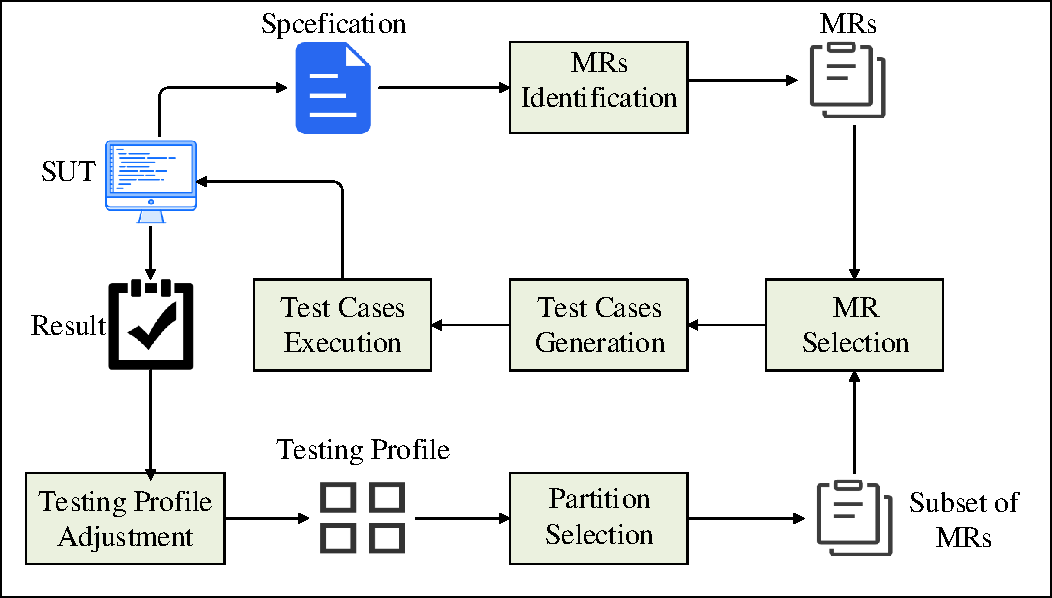
\includegraphics[width = 0.47\textwidth]{figs//framework//framework}
  \caption{DRT for web services framework}
  \label{fig:framework}
\end{figure}

It has been pointed out that fault-detecting inputs tend to cluster into ``continuous regions'' \cite{ammann1988data, finelli1991nasa}, that is, the test cases in some partition are more likely to detect faults than the test cases in other partitions. Following the above idea, AMT source test cases and MRs selection are in accordance with the testing profile that is dynamically updated during the test process. In our study, the strategies updating test profile, have been described in Section \ref{section:drtandmdrt}.

\subsection{Two Strategies of Updating Testing Profile}
\label{section:drtandmdrt}

\subsubsection{Dynamic Random Testing}
\label{section:drt}
Dynamic Random Testing (DRT) \cite{cai2009random} combines RT and PT, with the goal of benefitting from the advantages of both. Given a test suite $TS$ classified into $m$ ($m \ge 2$) partitions (denoted $s_1, s_2, \ldots, s_m$), and DRT is employed to update the values of the selection probabilities $p_i$. Assume that a source test case $stc$ from $s_i$ ($i = 1, 2, \ldots, m$) is selected, and an metamorphic relation $MR_h$ that is selected according to some strategies, is used to generate follow-up test case $ftc$ from $stc$. If $stc$ and $ftc$ belong to $s_i$, and their results violate the $MR_h$, $\forall j = 1, 2, \ldots, m$ and $j \neq i$, we then set

\begin{equation}
\label{eq:DRThitJ}
%\text{new} p_j =
p'_j =
\begin{cases}
p_j - \displaystyle\frac{\epsilon}{m-1} & \text{if } p_j \geq \displaystyle\frac{\epsilon}{m-1} \\
0 & \text{if } p_j < \displaystyle\frac{\epsilon}{m-1}
\end{cases},
\end{equation}
where $\epsilon$ is a probability adjusting factor, and then

\begin{equation}
\label{eq:DRThitI}
  p'_i = 1 - \sum_{\substack{j = 1 \\ j \neq i}}^m p'_j.
\end{equation}

Alternatively, if their results hold the $MR_h$, we set

\begin{equation}
\label{eq:DRTmissI}
%\text{new } p_i =
p'_i =
\begin{cases}
p_i - \epsilon & \text{if } p_i \geq \epsilon \\
0 & \text{if } p_i < \epsilon
\end{cases},
\end{equation}
and then for $\forall j = 1, 2, \ldots, m$ and $j \neq i$, we set

\begin{equation}
\label{eq:DRTmissJ}
p'_j =
\begin{cases}
p_j + \displaystyle\frac{\epsilon}{m-1} & \text{if } p_i \geq \epsilon \\
p_j + \displaystyle\frac{p'_i}{m-1} & \text{if } p_i < \epsilon
\end{cases}.
\end{equation}

 The detailed DRT algorithm is given in Algorithm \ref{alg:drt}. In DRT, the source test case is selected from a partition that has been randomly selected according to the testing profile $\{\left \langle s_1, p_1 \right \rangle, \left \langle s_2, p_2 \right \rangle, \ldots, \left \langle s_m, p_m \right \rangle\}$, and an metamorphic relation is select according to some strategies (Lines 2 to 4 in Algorithm \ref{alg:drt}). During the testing, if the source and follow-up test cases are belonging to same partition, then the testing profile is updated by changing the $p_i$: If a fault is detected, then Formulas \ref{eq:DRThitJ} and \ref{eq:DRThitI} are used to adjust the values of $p_i$ (Line 8), otherwise Formulas \ref{eq:DRTmissI} and \ref{eq:DRTmissJ} are used (Line 10). This process is repeated until a termination condition is satisfied (Line 1). Examples of termination conditions can be ``when the testing resources are exhausted,'' ``when a certain number of test cases have been executed,'' ``when the first faults is detected,'' etc.

\begin{algorithm}
\caption{DRT}
\label{alg:drt}
    \begin{algorithmic}[1]
    \renewcommand{\algorithmicrequire}{\textbf{Input:}}
    \renewcommand{\algorithmicendwhile}{\algorithmicend\_\algorithmicwhile}
    \renewcommand{\algorithmicendif}{\algorithmicend\_\algorithmicif}
    \REQUIRE $\epsilon, p_1, p_2, \ldots, p_m, MR_1, MR_2, \ldots, MR_n$
    \WHILE {termination condition is not satisfied}
    \STATE Select a partition $s_i$ according to the testing profile $\{\left \langle s_1, p_1 \right \rangle, \left \langle s_2, p_2 \right \rangle, \ldots, \left \langle s_m, p_m \right \rangle\}$.
    \STATE Select a source test case $stc$ from $s_i$, and an metamorphic relation $MR_h$ ($h \in \{1, 2, \ldots, n\}$).
    \STATE $MR_h$ is used to generate follow-up test case $ftc$ from $stc$.
    \STATE Test the SUT using $stc$ and $ftc$.
    \IF {both $stc$ and $ftc$ belong to $s_i$}
    \IF {the results of $stc$ and $ftc$ violate the MR}
    \STATE Update $\{\left \langle s_1, p_1 \right \rangle, \left \langle s_2, p_2 \right \rangle, \ldots, \left \langle s_m, p_m \right \rangle\}$ according to Formulas \ref{eq:DRThitJ} and \ref{eq:DRThitI}.
    \ELSE
    \STATE Update $\{\left \langle s_1, p_1 \right \rangle, \left \langle s_2, p_2 \right \rangle, \ldots, \left \langle s_m, p_m \right \rangle\}$ according to Formulas \ref{eq:DRTmissI} and \ref{eq:DRTmissJ}
    \ENDIF
    \ENDIF
    \ENDWHILE
    \end{algorithmic}
\end{algorithm}

\subsubsection{Metamorphic Dynamic Random Testing}
\label{section:mdrt}

When the source test case $stc_i$ and follow-up test case $ftc_i$ related to an metamorphic relation $MR_h$ belong to same partition $s_i$, DRT is suitable to adjust the testing profile. However, during the testing process, there are some scenarios where the $stc_i$ is not in the same partition as $ftc_i$. In such scenarios, DRT cannot be used to adjust the testing profile. To solve this problem, a new strategy, named  Metamorphic Dynamic Random Testing (MDRT), is proposed.

In MDRT, we consider the scenarios, in which source test case $stc$ and follow-up test case $ftc$ related to an metamorphic relation $MR_h$, belong to $s_i$ and $s_f$ ($f \in \{1, 2, \ldots, m\}, f \ne i$), respectively. Suppose that $stc$ and $ftc$ is executed. If their results violate the $MR_h$, $\forall j = 1, 2, \ldots, m$ and $j \ne i, f$, we set

\begin{equation}
\label{eq:MDRThitJ}
p'_j =
\begin{cases}
p_j - \displaystyle\frac{2\epsilon}{m-2} & \text{if } p_j \geq \displaystyle\frac{2\epsilon}{m-2} \\
0 & \text{if } p_j < \displaystyle\frac{2\epsilon}{m-2}
\end{cases},
\end{equation}
where $\epsilon$ is a probability adjusting factor, and then

\begin{equation}
\label{eq:MDRThitI}
  p'_i = p_i + \displaystyle\frac{(1-\sum_{\substack{j = 1, j \ne i,m}}^m p_j^{'}) - p_i - p_f}{2},
\end{equation}

\begin{equation}
\label{eq:MDRThitF}
  p'_f = p_f + \displaystyle\frac{(1-\sum_{\substack{j = 1, j \ne i,m}}^m p_j^{'}) - p_i - p_f}{2}.
\end{equation}

Alternatively, if their results hold the $MR_h$, we set

\begin{equation}
\label{eq:MDRTmissI}
p'_i =
\begin{cases}
p_i - \epsilon & \text{if } p_i \geq \epsilon \\
0 & \text{if } p_i < \epsilon
\end{cases},
\end{equation}

\begin{equation}
\label{eq:MDRTmissF}
p'_f =
\begin{cases}
p_f - \epsilon & \text{if } p_f \geq \epsilon \\
0 & \text{if } p_f < \epsilon
\end{cases},
\end{equation}
and then for $\forall j = 1, 2, \ldots, m$ and $j \neq i, f$, we set

\begin{equation}
\label{eq:MDRTmissJ}
p'_j = p_j + \displaystyle\frac{(p_i - p_i^{'}) + (p_f - p_f^{'})}{m - 2}
\end{equation}

The detailed MDRT algorithm is given in Algorithm \ref{alg:mdrt}. In MDRT, the source test case is selected from a partition that has been randomly selected according to the testing profile $\{\left \langle s_1, p_1 \right \rangle, \left \langle s_2, p_2 \right \rangle, \ldots, \left \langle s_m, p_m \right \rangle\}$, and an metamorphic relation is select according to some strategies (Lines 2 to 4 in Algorithm \ref{alg:drt}). During the testing, if the source and follow-up test cases are not in same partition, then the testing profile is updated by changing the $p_i$: If a fault is detected, then Formulas \ref{eq:MDRThitJ}, \ref{eq:MDRThitI}, and \ref{eq:MDRThitF} are used to adjust the values of $p_i$ (Line 8), otherwise Formulas \ref{eq:MDRTmissI}, \ref{eq:MDRTmissF}, and \ref{eq:MDRTmissJ} are used (Line 10). The testing process is stopped as long as the termination condition is satisfied.  

\begin{algorithm}
\caption{MDRT}
\label{alg:mdrt}
    \begin{algorithmic}[1]
    \renewcommand{\algorithmicrequire}{\textbf{Input:}}
    \renewcommand{\algorithmicendwhile}{\algorithmicend\_\algorithmicwhile}
    \renewcommand{\algorithmicendif}{\algorithmicend\_\algorithmicif}
    \REQUIRE $\epsilon, p_1, p_2, \ldots, p_m, MR_1, MR_2, \ldots, MR_n$
    \WHILE {termination condition is not satisfied}
    \STATE Select a partition $s_i$ according to the testing profile $\{\left \langle s_1, p_1 \right \rangle, \left \langle s_2, p_2 \right \rangle, \ldots, \left \langle s_m, p_m \right \rangle\}$.
    \STATE Select a source test case $stc_i$ from $s_i$, and an metamorphic relation $MR_h$ ($h \in \{1, 2, \ldots, n\}$).
    \STATE Based on the $MR_h$, follow-up test case $ftc_i$ is generated from $stc_i$, belonging to partition $s_f$.
    \STATE Test the SUT using $stc_i$ and $ftc_i$.
    \IF {$i \ne f$}
    \IF {the results of $stc_i$ and $ftc_i$ violate the MR}
    \STATE Update $\{\left \langle s_1, p_1 \right \rangle, \left \langle s_2, p_2 \right \rangle, \ldots, \left \langle s_m, p_m \right \rangle\}$ according to Formulas \ref{eq:MDRThitJ}, \ref{eq:MDRThitI}, and \ref{eq:MDRThitF}.
    \ELSE
    \STATE Update $\{\left \langle s_1, p_1 \right \rangle, \left \langle s_2, p_2 \right \rangle, \ldots, \left \langle s_m, p_m \right \rangle\}$ according to Formulas \ref{eq:MDRTmissI}, \ref{eq:MDRTmissF}, and \ref{eq:MDRTmissJ}.
    \ENDIF
    \ENDIF
    \ENDWHILE
    \end{algorithmic}
\end{algorithm}
\subsection{M-AMT}
\label{section:m-amt}
several independent researchers from different areas have individually observed that the fault-detecting inputs tend to cluster into ``continuous regions'' \cite{ammann1988data, finelli1991nasa}, which indicates  that if a fault is detected by a test case in a partition $s_i$, the execution of more tests from $s_i$ will more likely lead to fault detection. Based above observation, M-AMT attempts to give a higher chance to the fault-detecting MRs and test cases.


\subsection{Prototype}
\label{section:propotype}




\section{Empirical Study}
\label{section:empirical}

\subsection{Research Questions}
\label{section:questions}

\subsection{Object Programs}

\section{Related Work}
\label{section:related}

\subsection{Metamorphic Testing}

\subsection{Danymic Random Testing}
Cai et al. introduced software cybernetics \cite{cai2002optimal} to software testing, and proposed Adaptive Testing (AT) \cite{Cai07, hu2005case, hu2009improved}, which takes
advantage of feedback information to control the execution process, has been shown that AT outperforms RT in terms of T-measure and increasing the number of faults, which means
that AT has higher efficiency and effectiveness than RT.

\section*{Acknowledgment}

\newcommand{\BIBdecl}{\setlength{\itemsep}{0.2 em}}

\bibliographystyle{IEEEtran}
\bibliography{AMT}


\end{document}
